\section{(1.b)}
The parameters for the function rand() below are adopted from the Numerical Recipes book. After testing combinations of random generators A with C/D ( as stated in the book), we chose the combination A1C1 as the optimized choice.
\begin{figure}[!htb]
  \centering
  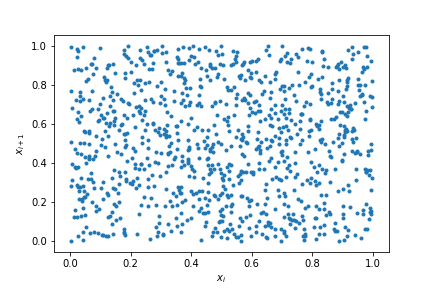
\includegraphics[width=0.7\linewidth]{Plots/scatt_1b.png}
  \caption{The scatter plot of generated random numbers}
  \label{fig:fig1}
\end{figure}

\begin{figure}[!htb]
  \centering
  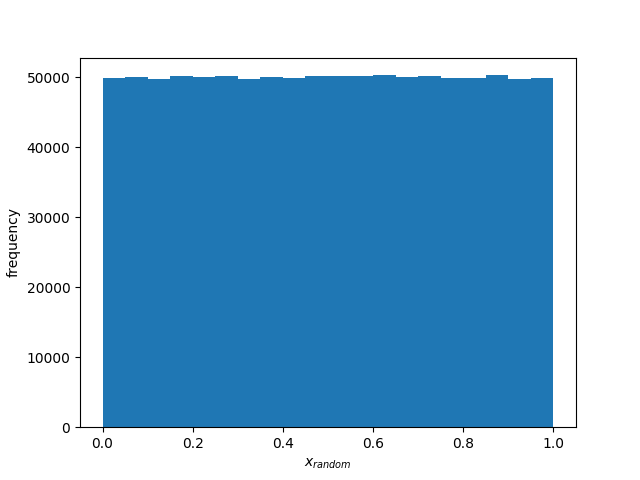
\includegraphics[width=0.7\linewidth]{Plots/hist_1b.png}
  \caption{The distribution of random numbers with equally spaced bins}
  \label{fig:fig2}
\end{figure}

As the Fig. 1 shows, the generated numbers are uncorrelated and well randomly distributed but some of the spots are not generated well. (sadly!\\
As Fig. 2 shows, all the numbers in the bins are produced almost equally probable.

\lstinputlisting{one_b.py}



